%% Creator: Inkscape inkscape 0.48.0, www.inkscape.org
%% PDF/EPS/PS + LaTeX output extension by Johan Engelen, 2010
%% Accompanies image file 'ids-erd.eps' (pdf, eps, ps)
%%
%% To include the image in your LaTeX document, write
%%   \input{<filename>.pdf_tex}
%%  instead of
%%   \includegraphics{<filename>.pdf}
%% To scale the image, write
%%   \def\svgwidth{<desired width>}
%%   \input{<filename>.pdf_tex}
%%  instead of
%%   \includegraphics[width=<desired width>]{<filename>.pdf}
%%
%% Images with a different path to the parent latex file can
%% be accessed with the `import' package (which may need to be
%% installed) using
%%   \usepackage{import}
%% in the preamble, and then including the image with
%%   \import{<path to file>}{<filename>.pdf_tex}
%% Alternatively, one can specify
%%   \graphicspath{{<path to file>/}}
%% 
%% For more information, please see info/svg-inkscape on CTAN:
%%   http://tug.ctan.org/tex-archive/info/svg-inkscape

\begingroup
  \makeatletter
  \providecommand\color[2][]{%
    \errmessage{(Inkscape) Color is used for the text in Inkscape, but the package 'color.sty' is not loaded}
    \renewcommand\color[2][]{}%
  }
  \providecommand\transparent[1]{%
    \errmessage{(Inkscape) Transparency is used (non-zero) for the text in Inkscape, but the package 'transparent.sty' is not loaded}
    \renewcommand\transparent[1]{}%
  }
  \providecommand\rotatebox[2]{#2}
  \ifx\svgwidth\undefined
    \setlength{\unitlength}{633.2pt}
  \else
    \setlength{\unitlength}{\svgwidth}
  \fi
  \global\let\svgwidth\undefined
  \makeatother
  \begin{picture}(1,0.58117498)%
    \put(0,0){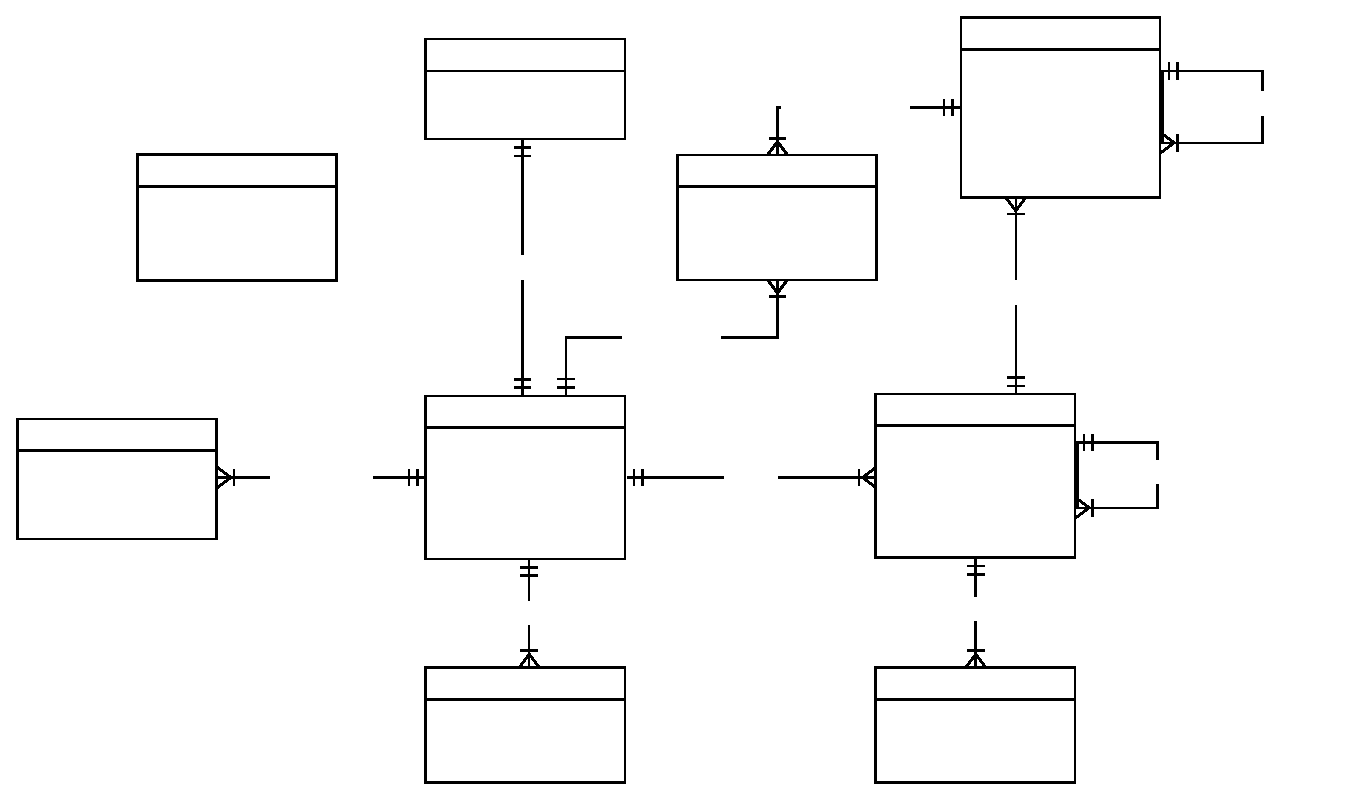
\includegraphics[width=\unitlength]{erd.eps}}%
    \put(0.38597599,0.54832596){\makebox(0,0)[b]{\smash{Status}}}%
    \put(0.38597599,0.52116235){\makebox(0,0)[b]{\smash{Is\_Connected}}}%
    \put(0.38597599,0.27771636){\makebox(0,0)[b]{\smash{Client}}}%
    \put(0.38597599,0.25055275){\makebox(0,0)[b]{\smash{Client\_Id}}}%
    \put(0.38597599,0.23185407){\makebox(0,0)[b]{\smash{Hostname}}}%
    \put(0.38597599,0.2131554){\makebox(0,0)[b]{\smash{Secret\_Key}}}%
    \put(0.79153506,0.56475047){\makebox(0,0)[b]{\smash{Version}}}%
    \put(0.79153506,0.53758686){\makebox(0,0)[b]{\smash{Version\_Id}}}%
    \put(0.79153506,0.51888819){\makebox(0,0)[b]{\smash{Backed\_Up\_At}}}%
    \put(0.79153506,0.50018951){\makebox(0,0)[b]{\smash{Mtime}}}%
    \put(0.79153506,0.48149084){\makebox(0,0)[b]{\smash{Size}}}%
    \put(0.79153506,0.46279217){\makebox(0,0)[b]{\smash{Hash}}}%
    \put(0.72710044,0.27921668){\makebox(0,0)[b]{\smash{Item}}}%
    \put(0.72710044,0.25205306){\makebox(0,0)[b]{\smash{Item\_Id}}}%
    \put(0.72710044,0.23335439){\makebox(0,0)[b]{\smash{Name}}}%
    \put(0.72710044,0.21465572){\makebox(0,0)[b]{\smash{Type}}}%
    \put(0.72710044,0.19595704){\makebox(0,0)[b]{\smash{Path}}}%
    \put(0.72710044,0.17725837){\makebox(0,0)[b]{\smash{Is\_Deleted}}}%
    \put(0.75742262,0.36702464){\makebox(0,0)[b]{\smash{Contains}}}%
    \put(0.38344915,0.38585755){\makebox(0,0)[b]{\smash{Has}}}%
    \put(0.23120657,0.22931143){\makebox(0,0)[b]{\smash{Backs up}}}%
    \put(0.07643714,0.26026532){\makebox(0,0)[b]{\smash{File Path}}}%
    \put(0.07643714,0.23310171){\makebox(0,0)[b]{\smash{Path}}}%
    \put(0.38597599,0.07201516){\makebox(0,0)[b]{\smash{Exclusion}}}%
    \put(0.38597599,0.04485155){\makebox(0,0)[b]{\smash{Pattern}}}%
    \put(0.38850284,0.12393399){\makebox(0,0)[b]{\smash{Excludes}}}%
    \put(0.72710044,0.07201516){\makebox(0,0)[b]{\smash{Event}}}%
    \put(0.72710044,0.04485155){\makebox(0,0)[b]{\smash{Occured\_At}}}%
    \put(0.72710044,0.02615287){\makebox(0,0)[b]{\smash{Type}}}%
    \put(0.576753,0.46050814){\makebox(0,0)[b]{\smash{RestoreJob}}}%
    \put(0.576753,0.43334452){\makebox(0,0)[b]{\smash{Created\_At}}}%
    \put(0.576753,0.41464585){\makebox(0,0)[b]{\smash{Started\_At}}}%
    \put(0.576753,0.39594718){\makebox(0,0)[b]{\smash{Completed\_At}}}%
    \put(0.49633311,0.33543904){\makebox(0,0)[b]{\smash{Restores}}}%
    \put(0.62823259,0.50979154){\makebox(0,0)[b]{\smash{Restored by}}}%
    \put(0.94440935,0.5102969){\makebox(0,0)[b]{\smash{Restored from}}}%
    \put(0.86481364,0.23108023){\makebox(0,0)[b]{\smash{Child of}}}%
    \put(0.72710044,0.1269741){\makebox(0,0)[b]{\smash{Has}}}%
    \put(0.55653822,0.22931143){\makebox(0,0)[b]{\smash{Has}}}%
    \put(0.16740366,0.46083386){\makebox(0,0)[b]{\smash{GlobalExclusion}}}%
    \put(0.16740366,0.43367025){\makebox(0,0)[b]{\smash{Pattern}}}%
  \end{picture}%
\endgroup
